\chapter{Algorithms}
\label{chapter:algs}

The main focus of this thesis is on improving the performance of small matrix multiplication algorithms. It is necessary to finesse around the bottlenecks that constrain the approaches described in the previous chapter. The extra information which makes this possible is the sparsity pattern known at compile time. The focus is on dense-by-sparse multiplication because it stands to benefit the most from vectorization, although sparse-by-dense and tensor-by-sparse multiplication are also discussed. Figure~\ref{fig:dxspfamilies} shows the different dense-by-sparse algorithms under consideration and the relationships between them. 

The starting point is the dense outer-product formulation generated from \texttt{libxsmm}. Applying knowledge about the sparsity pattern yields MicroSparse, which avoids wasted computation but is restricted to very small matrix sizes. Decomposing a matrix into blocks, using MicroSparse for each block, and unrolling some of the outer loops yields UnrolledSparse, which is not restricted by matrix dimensions but is restricted by the number of nonzeros. In order to support matrices with many nonzeros, some regularity assumptions have to be made. 

\begin{figure}[tbh]
  \centering
  

\usetikzlibrary{shapes,arrows}
\usetikzlibrary{decorations.pathreplacing}


% Define block styles
\tikzstyle{decision} = [diamond, draw, fill=blue!20, 
    text width=4.5em, text badly centered, node distance=3cm, inner sep=0pt]

\tikzstyle{block} = [rectangle, draw, fill=gray!20, 
    text width=7em, text centered, minimum height=3em]

\tikzstyle{line} = [draw, -latex']

\tikzstyle{cloud} = [draw, ellipse,fill=red!20, node distance=3cm,
    minimum height=2em]

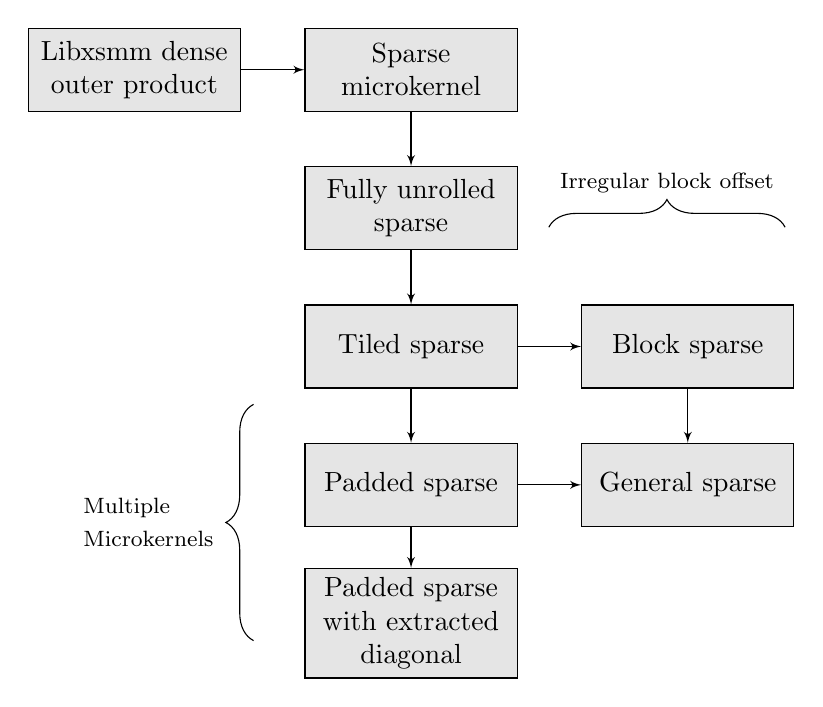
\begin{tikzpicture}[node distance = 5em, auto]
    % Place nodes

    \node [block] (microkernel) {Sparse\\ microkernel};
    \node [block, left of=microkernel, node distance=10em] (libxsmm) {Libxsmm dense outer product};
    \node [block, below of=microkernel] (macrokernel) {Fully unrolled\\ sparse};
    \node [block, below of=macrokernel] (tiledsparse) {Tiled sparse};
    \node [block, right of=tiledsparse, node distance=10em] (blocksparse) {Block sparse};
    \node [block, below of=tiledsparse] (paddedsparse) {Padded sparse};
    \node [block, below of=blocksparse] (generalsparse) {General sparse};
    \node [block, below of=paddedsparse] (paddeddiagsparse) {Padded sparse with extracted diagonal};

    %\node [block, left of=evaluate, node distance=3cm] (update) {update model};
    %\node [decision, below of=evaluate] (decide) {is best candidate better?};
    %\node [block, below of=decide, node distance=3cm] (stop) {stop};

    % Draw edges
    \path [line] (libxsmm) -- (microkernel);
    \path [line] (microkernel) -- (macrokernel);
    \path [line] (macrokernel) -- (tiledsparse);
    \path [line] (tiledsparse) -- (blocksparse);
    \path [line] (tiledsparse) -- (paddedsparse);
    \path [line] (paddedsparse) -- (generalsparse);
    \path [line] (blocksparse) -- (generalsparse);
    \path [line] (paddedsparse) -- (paddeddiagsparse);

    \draw [decorate,decoration={brace,amplitude=10pt},xshift=0pt,yshift=0pt]
(1.75,-2) -- (4.75,-2)node [black,midway,yshift=9pt] {\footnotesize Irregular block offset};

    \draw [decorate,decoration={brace,amplitude=10pt},xshift=0pt,yshift=0pt]
(-2,-7.25) -- (-2,-4.25) node [black,midway,xshift=-8pt,text width=5em] {\footnotesize Multiple\\ Microkernels};
    %\path [line] (evaluate) -- (decide);
    %\path [line] (decide) -| node [near start] {yes} (update);
    %\path [line] (update) |- (identify);
    %\path [line] (decide) -- node {no}(stop);
    %\path [line,dashed] (expert) -- (init);
    %\path [line,dashed] (system) -- (init);
    %\path [line,dashed] (system) |- (evaluate);
\end{tikzpicture}



  \caption{Relationships between different dense-by-sparse multiplication algorithms}
  \label{fig:dxspfamilies}
\end{figure}


The simplest approach is TiledSparse, which assumes that a single block pattern is repeated exactly. This assumption is impractical because for most matrix patterns, the block pattern will fill in. Instead we can break the assumption into two parts and relax them separately. We can assume that there is only one block sparsity pattern, but some blocks are entirely zero, which yields the BlockSparse algorithm. Alternatively, we can assume that there are multiple block sparsity patterns, but they all have the same number of nonzeros, which yields PatternSparse. Relaxing both assumptions yields GeneralSparse, which can evade the number of nonzeros constraint with the most flexibility, but at the cost of additional overhead. Variations can be explored which extract the diagonal and handle it separately; this would be especially helpful for PaddedSparse in the case of matrices with a full diagonal and random fill-in elsewhere.

\section{Dense-by-sparse microkernel}

The MicroSparse kernel is our first attempt to account for the sparsity pattern while building off of the state of the art for dense matrix multiplication. Our key assumption is that the matrices A and C are small enough to fit entirely in registers: $(n + k) * (m/8) <= 32$. Generating the dense GEMM for this problem effectively extracts the dense microkernel. This microkernel has no loops (otherwise it couldn't amortize the cost of loading and storing A and C) and this makes it easy to modify.

The sparse microkernel is a straightforward modification of the dense microkernel. All FMA instructions \py{C[:,ni] += A[:,ki] .* B[ki, ni]} where \py{B[ki, ni] = 0} due to the sparsity pattern are removed. This is tricky to do in a general way; an abstraction designed for the purpose is described at length in Section X.XX. Next, any loads of a column of A corresponding to an empty row of B are removed. Finally, any loads and stores of a column of C corresponding to an empty column of B are removed. This is described via pseudocode in Figure~\ref{fig:micropseudo}.

\begin{figure}[htb]
\centering
  \begin{minted}[linenos=false,fontsize=\footnotesize]{text}

    for each vector Vmi:
        for each cell ni:
            if B[:,ni] != 0:
                emit load C[Vmi, ni]

    for each vector Vmi:
        for each cell ki:
            if B[ki,:] != 0:
                emit load A[Vmi, ki]

    for each vector Vmi:
        for each cell ki:
            for each cell ni:
                if B[ki,ni] != 0:
                    emit fma C[Vmi, ni] += A[Vmi, ki] .* B[ki, ni]

    for each vector Vmi:
        for each cell ni:
            if B[:,ni] != 0:
                emit store C[Vmi, ni]

  \end{minted}
  \caption{Pseudocode for UnrolledSparse}
\label{fig:micropseudo}
\end{figure}

Before proceeding to more complex algorithms, it is worthwhile to consider the degrees of freedom available. The first parameter to consider is the format of the sparse matrix B. Because the memory offsets of each \py{B[ki,ni]} are hardcoded into the FMA, any format will work as long as the pointer to B never moves. However, the choice of format strongly affects memory access patterns. Keeping B dense is suboptimal because the algorithm will be streaming nonzeros which are unduly spread across different cache lines. Breuer and Heinecke used a virtual compressed sparse column format, where the nonzeros were laid out in a plain 1D array ordered by columns. For SparseMicrokernel, a virtual compressed row format might have better locality because the $ni$ loop is innermost, but this is insignificant because few cache lines are involved on sparse matrices of this size. 

Having chosen the format, the next step is to choose the addressing mode for the elements of the sparse matrix. For now we assume that B points to the first entry in this matrix and the entries are all adjacent. Because the maximum number of doubles in B is 256 and the cutoff for 7-byte FMAs is 128, it already makes sense to switch to scale-index addressing. Because this is complicated to do, it will be hidden behind an abstraction detailed in Section X.XX.

Another question is alignment. The alignment of B is not particularly important because its elements are loaded one at a time, but very important for A and C, which are loaded in a vectorwise fashion. If not aligned on a 64-byte boundary, the vector load operation will suffer a delay because the data is split across two cache lines. Using the aligned vector load operation \py{vmovapd} will trigger a segmentation fault if the pointer is not actually aligned. On the other hand, the unaligned version \py{vmovupd} can handle both the aligned and unaligned case, and will not incur the penalty if the pointer is in fact aligned. Fortunately, this choice can be made independently of any other considerations.

The performance of SparseMicrokernel shall be explored in Section X.XX. It is clear that removing the FMA instructions decreases the arithmetic intensity, and if the nonzeros are evenly distributed, there will be no accompanying decrease in memory bandwidth. Nevertheless the algorithm remains compute-bound and experiences an improved time-to-solution compared to its dense counterpart. Regardless of performance, SparseMicrokernel has limited utility in real problems, since it can only be applied to extremely small matrices. It is valuable primarily as a building block for the more complex algorithms developed next.


\section{Unrolled dense-by-sparse multiplication}


The goal of UnrolledSparse is to support larger matrix sizes by building off of MicroSparse. The first key idea is to introduce a block decomposition: the generators traverse blocks $(Bmi, Bni, Bki)$ and delegate the multiplication of each block to MicroSparse. The second key idea is to account for the fact that different blocks contain different subpatterns by unrolling the $Bni$ and $Bki$ loops. The sparsity pattern is obviously invariant with respect to $Bmi$, so it is not necessary to unroll that loop. 

It is essential that $Bki$ be the innermost loop because this lets us accumulate changes to the block \py{C[Bmi, Bni]}, and then store the entire block exactly once. Otherwise, the repeated storing of each block of C becomes the primary bottleneck. This also means that we only reuse the inner part of MicroSparse, and we handle the loads and stores of C ourselves.

Putting the $Bmi$ loop on the outside is the best choice for several reasons. Firstly, it consolidates instructions that are free of control dependencies, which improves pipeline efficiency and gives the processor more room to amortize loads of A and C. Secondly, it dramatically reduces the number of branches. Even if branches are predicted perfectly, KNL's issue-width bottleneck ensures that the instructions to increment and compare the counter register would displace FMAs, reducing performance.

Thus there is only one reasonable ordering for our loop nest. At the innermost level we unroll over the $Bki$ loop, laying down a sequence of sparse microkernels corresponding to a traversal of one panel of B, moving from top to bottom in short, fat slices. In the middle level, we unroll over $Bni$, corresponding to a traversal across panels of B from left to right. Finally, at the outermost level, we loop over $Bmi$: horizontal panels of A and C from top to bottom. This is described more precisely via pseudocode in Listing X.XX.

This loop nesting looks very similar to what Goto calls GEPM\_VAR2, depicted in Figure~\ref{fig:gepm}. Note that Goto rejects this algorithm within one paragraph, making the exact opposite argument as we have made above, regarding the repeated storing of the C block. This is because Goto is focusing on a much larger scale: his C blocks fit only in the L2 cache, whereas ours fit entirely in registers: we get our inner ``GEPDot'' for free whereas his is especially costly.

The UnrolledSparse algorithm has three additional tuning parameters which must be chosen. These are the blocksizes $bm$, $bn$, and $bk$. Section X.XX explores how to choose these values heuristically. The choice of parameters and the set of problems which can be efficiently solved are subject to the following constraints:

\begin{itemize}
  \item The A and C blocks must fit in registers: $(bk + bn) * (bm / 8) <= 32$
  
  \item Each nonzero in B produces exactly one FMA, and if there are too many of these, they will fill the instruction cache. This introduces a hard limit on the number of nonzeros, which shall be explored in depth in Section X.XX.
  
  \item The instruction cache bottleneck can be hit with fewer nonzeros depending on the choice of blocksizes, since different blocksizes result in different numbers of \py{vmovapd} instructions. This is explored in depth in Section X.XX.

  \item Choices of $(m,n,k)$ which do not evenly divide into small blocks are feasible, but not fully supported at the time of this writing.
\end{itemize}

The experiments discussed later consistently show that UnrolledSparse strikes a good balance between performance and flexibility. It supports most available matrix sizes, it does not fill in any zeros or waste any flops, and it uses a dense-style register blocking. It continues to perform well as the B matrix becomes dense -- the parallel efficiency increases -- and it degenerates to something similar to libxsmm. For fully dense matrices it performs slightly worse than libxsmm, and if it reaches the instruction cache limit it performs dramatically worse. In order to move past this constraint, we find ways to compress the number of FMAs below the number of actual nonzeros.

\begin{figure}[tb]
  \centering
  \begin{subfigure}[b]{0.32\textwidth}
    \centering
          \[
      \left[
          \begin{array}{c c c | c c c }
          0 &   &   & 10 &   &   \\
          1 & 2 &   & 11& 12&   \\
            & 3 & 4 &   & 13& 14  \\
          \hline
          5 &   &   & 15  &   &   \\
          6 & 7 &   & 16  &17   &   \\
            & 8 & 9 &   & 18  &19   \\
          \end{array}
          \right]
      \]
    \caption{TiledSparse}
    \label{fig:tiledblocks}
  \end{subfigure}
  \begin{subfigure}[b]{0.32\textwidth}
    \centering
      \[
      \left[
          \begin{array}{c c c | c c c }
          0 &   &   &    &    &    \\
          1 & 2 &   &    &    &    \\
            & 3 & 4 &    &    &    \\
          \hline
          5 &   &   & 10 &    &    \\
          6 & 7 &   & 11 & 12 &    \\
            & 8 & 9 &    & 13 & 14 \\
          \end{array}
          \right]
      \]    \caption{BlockedSparse}
    \label{fig:blockedblocks}
  \end{subfigure}
    \begin{subfigure}[b]{0.32\textwidth}
    \centering
      \[
      \left[
          \begin{array}{c c c | c c c }
          0 &   &   &    &    &    \\
          1 & 2 &   &    &    &    \\
            & 3 & 4 &    &    &    \\
          \hline
          5  & 6  & 7  &    &  14& 15  \\
          8  & 9  & 10 &    &    & 16 \\
          11 & 12 & 13 &    &    &    \\
          \end{array}
          \right]
      \]    \caption{GeneralSparse}
    \label{fig:generalblocks}
  \end{subfigure}
  \caption{Sample matrices illustrating the blocking constraints for different GEMM algorithms. TiledSparse admits only a single block pattern which is tiled perfectly over the entire matrix. BlockedSparse admits a single block pattern along with empty blocks. GeneralSparse relaxes further to admit multiple different patterns. The numbers indicate the cell's index when using a block compressed-sparse-row format. }
  \label{fig:matrixblocks}

\end{figure}




\begin{figure}[ht]
  \begin{subfigure}[b]{0.45\textwidth}
      \begin{minted}[linenos=false,fontsize=\footnotesize]{text}
        loop over m blocks:

           unroll loop over n blocks:

              load C block into registers

              unroll loop over k blocks:

                 load A block into registers
                 blockwise C += A * B
                 move A right 1 block
                 move B down 1 block

              store C block from registers
              move A to far left
              move B to top + right 1 block
              move C right 1 block

           move A down 1 block
           move C down 1 block
      \end{minted}    
      \caption{Pseudocode for UnrolledSparse}
    \label{fig:pseudocode_unrolled}
  \end{subfigure}
  ~~~~~~
  \begin{subfigure}[b]{0.45\textwidth}
      \begin{minted}[linenos=false,fontsize=\footnotesize]{text}
        loop over m blocks:

           loop over n blocks:

              load C block into registers

              unroll loop over k blocks:

                 load A block into registers
                 blockwise C += A * B
                 move A right 1 block
                 move B down 1 block

              store C block from registers
              move A to far left
              move B to top + right 1 block
              move C right 1 block

           move A down 1 block
           move C down 1 block
      \end{minted}    
      \caption{Pseudocode for TiledSparse}
    \label{fig:pseudocode_tiled}

  \end{subfigure}
    \caption{Pseudocode for UnrolledSparse and TiledSparse. UnrolledSparse unrolls two inner loops, emitting a microkernel for every block of B. TiledSparse unrolls only the innermost loop, emitting a microkernel for every (identical) block in one panel of B.}
    \label{fig:pseudocode_unrolled_tiled}

\end{figure}



\section{Tiled dense-by-sparse multiplication}

     The basic idea behind TiledSparse is to scale the FullyUnrolledSparse algorithm to 
matrices with more than 3100 nonzeros by assuming that the sparsity pattern is perfectly regular. 
Specifically, we assume that there is a single sparsity pattern which tiles over the entire matrix and is small enough to be used by MicroSparse. Our tiling assumption can be made without loss 
of generality because we can always fill in zeros until we arrive at a regular pattern. One
way to do this is to partition the original matrix with the desired blocksize, and then take the 
logical union of the sparsity patterns in each block. The assumption does result in a loss of 
practicality, however, as often the pattern will degenerate to dense. If the pattern becomes dense, the resulting algorithm will be more or less similar to libxsmm depending on the choice of block sizes.

There are several ways in which this algorithm may be modified.

The first design variable is the choice of loops to unroll. Because each block occupies the same amount of memory, the loops need only update the pointer to the current block, which makes unrolling very simple. The optimal amount of unrolling depends mainly on the number of nonzeros in the sparsity pattern. 

The second design variable is the representation of the sparse matrix in memory. The choice will
directly affect both memory locality and FMA instruction size. The assumption that it is possible to traverse the matrix block-by-block using simple pointer arithmetic constrains 
the feasible layouts to DNS, (V)CSR, and (V)CSC. The layout which best suits the 
memory accesses made by TiledSparse 
is VBCSR. If the layout is prescribed externally as something other than (V){BCSR, BCSC), 
or if the pattern contains more than 128 nonzeros, it is recommended to use multiple cursors in 
order to keep the FMA instruction size down. One possible interoperability trick is to store 
the matrix in COO format, but order the values according to VBCSR. Of course, this is fragile 
if the matrix gets modified.

As mentioned earlier, the main limitation to this algorithm is the tendency for the block pattern to 
fill in until it becomes mostly dense. Otherwise, it is limited to having fewer than ~3000 nonzeros 
in the pattern. It does not require the tiling to be perfect (where the bottommost and rightmost 
tiles are full sized), although this makes the generator more complicated and reduces the allowed 
number of nonzeros in the pattern to $3000 - nnz(top_right) - nnz(bottom_right) - nnz(bottom_left)$. 



        Assume there exists a sparse pattern which tiles perfectly over B.
        \begin{itemize}
        \item[$+$] We can reuse a single microkernel, reducing the number of instructions
        \item[$+$] We can visit blocks in a loop efficiently, using pointer tricks to reduce instruction size.
        \item[$-$] This regularity assumption is likely too strong.
        \item[$-$] In practice, the sparsity pattern would often become dense.
        \end{itemize}




\section{Block dense-by-sparse multiplication}

  Assume that B is decomposed into blocks which are either empty or `full'. `Full' blocks all have the same sparsity pattern. This is a sparse generalization of the block-sparse-column format.

  \begin{itemize}
  \item[$+$] We can reuse a single microkernel, reducing the number of instructions
  \item[$+$] The zero blocks reduce the number of filled-in nonzeros.
  \item[$-$] We can no longer visit blocks by using a loop with pointer arithmetic. \\Our options are:
    \begin{itemize}
    \item Look up the block location from a table in memory
    \item Unroll the block locations into the instruction stream and repeatedly jump to the microkernel.
    \end{itemize}
  \end{itemize}




* What are the performance bottlenecks?
* What sparse matrix format constraints?
* What block size constraints?
* On which matrices is this likely to be efficient? On which matrices is this likely to be inefficient?


\section{General dense-by-sparse multiplication}

The general dense-by-sparse algorithm comes from relaxing \emph{both} of the key ideas of TiledSparse: There can be any number of different block patterns, and each pattern may contain any number of nonzeros. GeneralSparse contains a collection of SparseMicrokernel GEMMs, and chooses the correct GEMM for each block of B. It is free to scale to larger matrix sizes than those supported by UnrolledSparse, because it can be compressed. Judiciously filling in zeros can arbitrarily reduce the number of unique block patterns, which in turn reduces the number of GEMMs. Thus GeneralSparse degrades gracefully, similar to TiledSparse. As the matrices grow larger and denser, the algorithm will converge towards either BlockedSparse or dense, depending on the original sparsity pattern. In contrast to TiledSparse and BlockedSparse, however, the fill-in (and hence wasted FLOPs) can be effectively minimized.

There is of course a tradeoff: in order to redirect control flow to the correct block GEMM, an indirect jump is needed. This introduces control dependencies and brings the branch predictor into play. For each indirect jump there will be additional latency, along with poorer memory movement amortization. There are several different strategies possible, each a modification which resolves problems introduced by the previous:

\begin{itemize}
  \item The first approach is a straightforward jump table. Suppose the different block GEMMs are numbered $0,1,...$. Then a \emph{jump table} can be laid out in the instruction stream. The address of each 


  \item Modify (1) to avoid the extra lookup by putting the address of the GEMM in the block array directly. Loop over this array, moving the \py{A,B,C} pointers to the start of the block, and performing an indirect jump to the GEMM at the address in the current array. Put all of the GEMMs in the center of the loop. There are three downsides to this approach: Firstly, each non-empty block has both an indirect jump (to the correct GEMM) and a direct jump (back to the body of the loop). Secondly, completely empty blocks still generate an indirect jump. Thirdly, there is no possibility of unrolling. This approach is explored in \py{src/jumptables/jumptable_looped.cpp}.

  \item Unroll the \py{Bn} and \py{Bk} loops completely. For each block, move the \py{A,B,C} pointers to the start of the active block, and save a return address to a register. This is effectively a (non-ABI-compliant) function call, except it avoids the stack completely. Perform a direct jump to the correct GEMM. The GEMM itself performs the indirect jump to the return address stored in the register. This approach is explored in \py{src/jumptables/jumptable_unrolled.cpp}.
\end{itemize}

\subsection{Pseudocode}


\subsection{Degrees of Freedom}
\begin{description}
  \item[Decision to unroll Bm-loop] 
  \item[Code alignment and padding]
\end{description}


\subsection{Constraints}

\begin{enumerate}

  \item The total number of indirect jumps should be minimized. This favors a larger block size.

  \item The routine must fit in the 32kB instruction cache, which constrains both the sum of nonzeros in each \emph{unique} block, as well as the total number of nonzero blocks. The latter constraint could possibly be finessed by storing the pointers to the start of each block and the corresponding GEMM routine in an array in the data cache instead of unrolling it into the instruction stream.

  \item The sparse matrix should be stored in \emph{block} compressed sparse row or column format in order to have good data locality.

  \item Blocks should be uniformly sized. This is an implementation detail; the constraint may be removed in the future by implementing another MatrixCursor as described in Section X.XX.

\end{enumerate}

\subsection{Choosing parameters}

How do we automatically choose GeneralSparse parameters?

\section{Sparse-by-dense multiplication}

One pattern which emerges in sparse matrices is to 

\section{Tensor-matrix multiplication}


